\documentclass[11pt,a4paper]{article}
%%%%%%%%%%%%%%%%%%%%%%%%% Credit %%%%%%%%%%%%%%%%%%%%%%%%

% template ini dibuat oleh martin.manullang@if.itera.ac.id untuk dipergunakan oleh seluruh sivitas akademik itera.

%%%%%%%%%%%%%%%%%%%%%%%%% PACKAGE starts HERE %%%%%%%%%%%%%%%%%%%%%%%%
\usepackage{graphicx}
\usepackage{caption}
\usepackage{microtype}
\captionsetup[table]{name=Tabel}
\captionsetup[figure]{name=Gambar}
\usepackage{tabulary}
\usepackage{minted}
% \usepackage{amsmath}
\usepackage{fancyhdr}
% \usepackage{amssymb}
% \usepackage{amsthm}
\usepackage{placeins}
% \usepackage{amsfonts}
\usepackage{graphicx}
\usepackage[all]{xy}
\usepackage{tikz}
\usepackage{verbatim}
\usepackage[left=2cm,right=2cm,top=3cm,bottom=2.5cm]{geometry}
\usepackage{hyperref}
\hypersetup{
    colorlinks,
    linkcolor={red!50!black},
    citecolor={blue!50!black},
    urlcolor={blue!80!black}
}
\usepackage{caption}
\usepackage{subcaption}
\usepackage{multirow}
\usepackage{psfrag}
\usepackage[T1]{fontenc}
\usepackage[scaled]{beramono}
% Enable inserting code into the document
\usepackage{listings}
\usepackage{xcolor} 
% custom color & style for listing
\definecolor{codegreen}{rgb}{0,0.6,0}
\definecolor{codegray}{rgb}{0.5,0.5,0.5}
\definecolor{codepurple}{rgb}{0.58,0,0.82}
\definecolor{backcolour}{rgb}{0.95,0.95,0.92}
\definecolor{LightGray}{gray}{0.9}
\lstdefinestyle{mystyle}{
	backgroundcolor=\color{backcolour},   
	commentstyle=\color{green},
	keywordstyle=\color{codegreen},
	numberstyle=\tiny\color{codegray},
	stringstyle=\color{codepurple},
	basicstyle=\ttfamily\footnotesize,
	breakatwhitespace=false,         
	breaklines=true,                 
	captionpos=b,                    
	keepspaces=true,                 
	numbers=left,                    
	numbersep=5pt,                  
	showspaces=false,                
	showstringspaces=false,
	showtabs=false,                  
	tabsize=2
}
\lstset{style=mystyle}
\renewcommand{\lstlistingname}{Kode}
%%%%%%%%%%%%%%%%%%%%%%%%% PACKAGE ends HERE %%%%%%%%%%%%%%%%%%%%%%%%


%%%%%%%%%%%%%%%%%%%%%%%%% Data Diri %%%%%%%%%%%%%%%%%%%%%%%%
\newcommand{\student}{\textbf{Dodi Rifai Sihombing (120140132)}}
\newcommand{\course}{\textbf{Sistem Operasi (IF2223)}}
\newcommand{\assignment}{\textbf{03}}

%%%%%%%%%%%%%%%%%%% using theorem style %%%%%%%%%%%%%%%%%%%%
\newtheorem{thm}{Theorem}
\newtheorem{lem}[thm]{Lemma}
\newtheorem{defn}[thm]{Definition}
\newtheorem{exa}[thm]{Example}
\newtheorem{rem}[thm]{Remark}
\newtheorem{coro}[thm]{Corollary}
\newtheorem{quest}{Question}[section]
%%%%%%%%%%%%%%%%%%%%%%%%%%%%%%%%%%%%%%%%
\usepackage{lipsum}%% a garbage package you don't need except to create examples.
\usepackage{fancyhdr}
\pagestyle{fancy}
\lhead{Dodi Rifai Sihombing (120140132)}
\rhead{ \thepage}
\cfoot{\textbf{Handson 3 : Docker}}
\renewcommand{\headrulewidth}{0.4pt}
\renewcommand{\footrulewidth}{0.4pt}

%%%%%%%%%%%%%%  Shortcut for usual set of numbers  %%%%%%%%%%%

\newcommand{\N}{\mathbb{N}}
\newcommand{\Z}{\mathbb{Z}}
\newcommand{\Q}{\mathbb{Q}}
\newcommand{\R}{\mathbb{R}}
\newcommand{\C}{\mathbb{C}}
\setlength\headheight{14pt}

%%%%%%%%%%%%%%%%%%%%%%%%%%%%%%%%%%%%%%%%%%%%%%%%%%%%%%%555
\begin{document}
\thispagestyle{empty}
\begin{center}
	
\includegraphics[scale = 0.15]{Figure/ifitera-header.png}
	\vspace{0.1cm}
\end{center}
\noindent
\rule{17cm}{0.2cm}\\[0.3cm]
Nama: \student \hfill Tugas Ke: \assignment\\[0.1cm]
Mata Kuliah: \course \hfill Tanggal: 02/05/2022\\
\rule{17cm}{0.05cm}
\vspace{0.1cm}



%%%%%%%%%%%%%%%%%%%%%%%%%%%%%%%%%%%%%%%%%%%%% BODY DOCUMENT %%%%%%%%%%%%%%%%%%%%%%%%%%%%%%%%%%%%%%%%%%%%%
\section{Tujuan HandsOn}
Tujuan dari HandsOn kali ini adalah agar mahasiswa dapat memahami tentang cara kerja Docker dan mengetahui serta memahami perintah-perintah dasar yang digunakan dalam Docker tersebut.


\section{Instalisasi}
Pada HandsOn kali ini hal pertama yang dilakukan adalah mendownload dan menginstal Docker terlebih dahulu melalui website docker.com, disini saya menggunakan windows maka saya menginstal Docker untuk versi windows.
\subsection{Requirements}
\begin{figure}[h]
        \centering
        \begin{subfigure}[b]{0.4\textwidth}
            \centering
            \def\svgwidth{\columnwidth}
            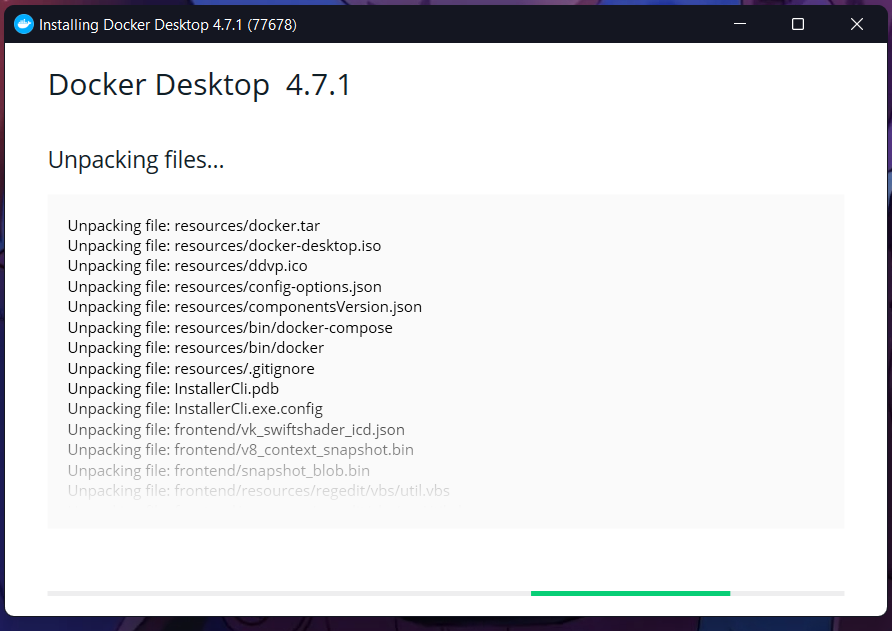
\includegraphics[width=1\textwidth]{Figure/instal docker.png}
        \end{subfigure}
        \qquad %add desired spacing between images, e. g. ~, \quad, \qquad, \hfill etc. 
        %(or a blank line to force the subfigure onto a new line)
        \begin{subfigure}[b]{0.4\textwidth}
            \centering
            \def\svgwidth{\columnwidth}
            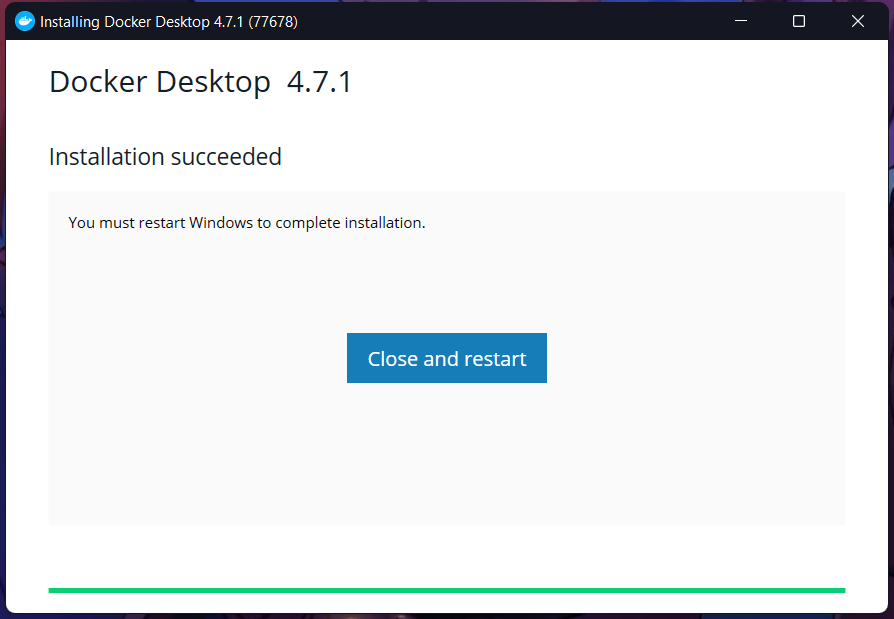
\includegraphics[width=1\textwidth]{Figure/instal done.png}
        \end{subfigure}
        \caption{Menginstal Docker}\label{fig:aug}
    \end{figure}

\begin{figure}[h]
	\centering
	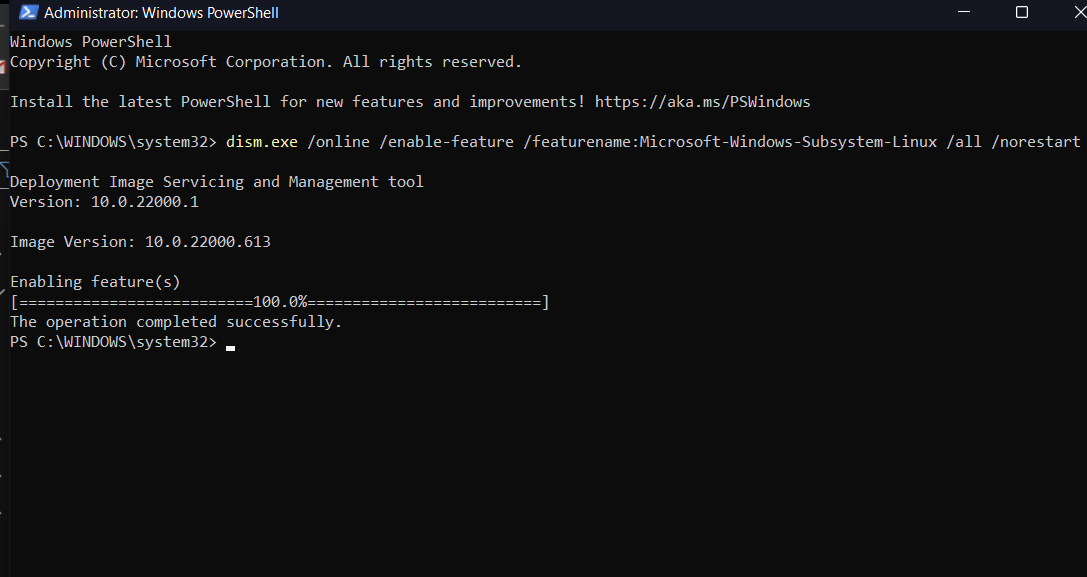
\includegraphics[width = 0.7\textwidth]{Figure/instal wsl2.png} .png}
	\caption{Instalasi Manual WSL2 dengan Windows PowerShell}
\end{figure}
\newpage
Disini docker masih belum bisa digunakan karena docker membutuhkan wsl2. Windows Subsystem for Linux (WSL) merupakan sistem operasi yang dikembangkan oleh Microsoft agar pengguna dari Windows dapat menjalankan
aplikasi berbasis linux.

\begin{figure}[h]
	\centering
	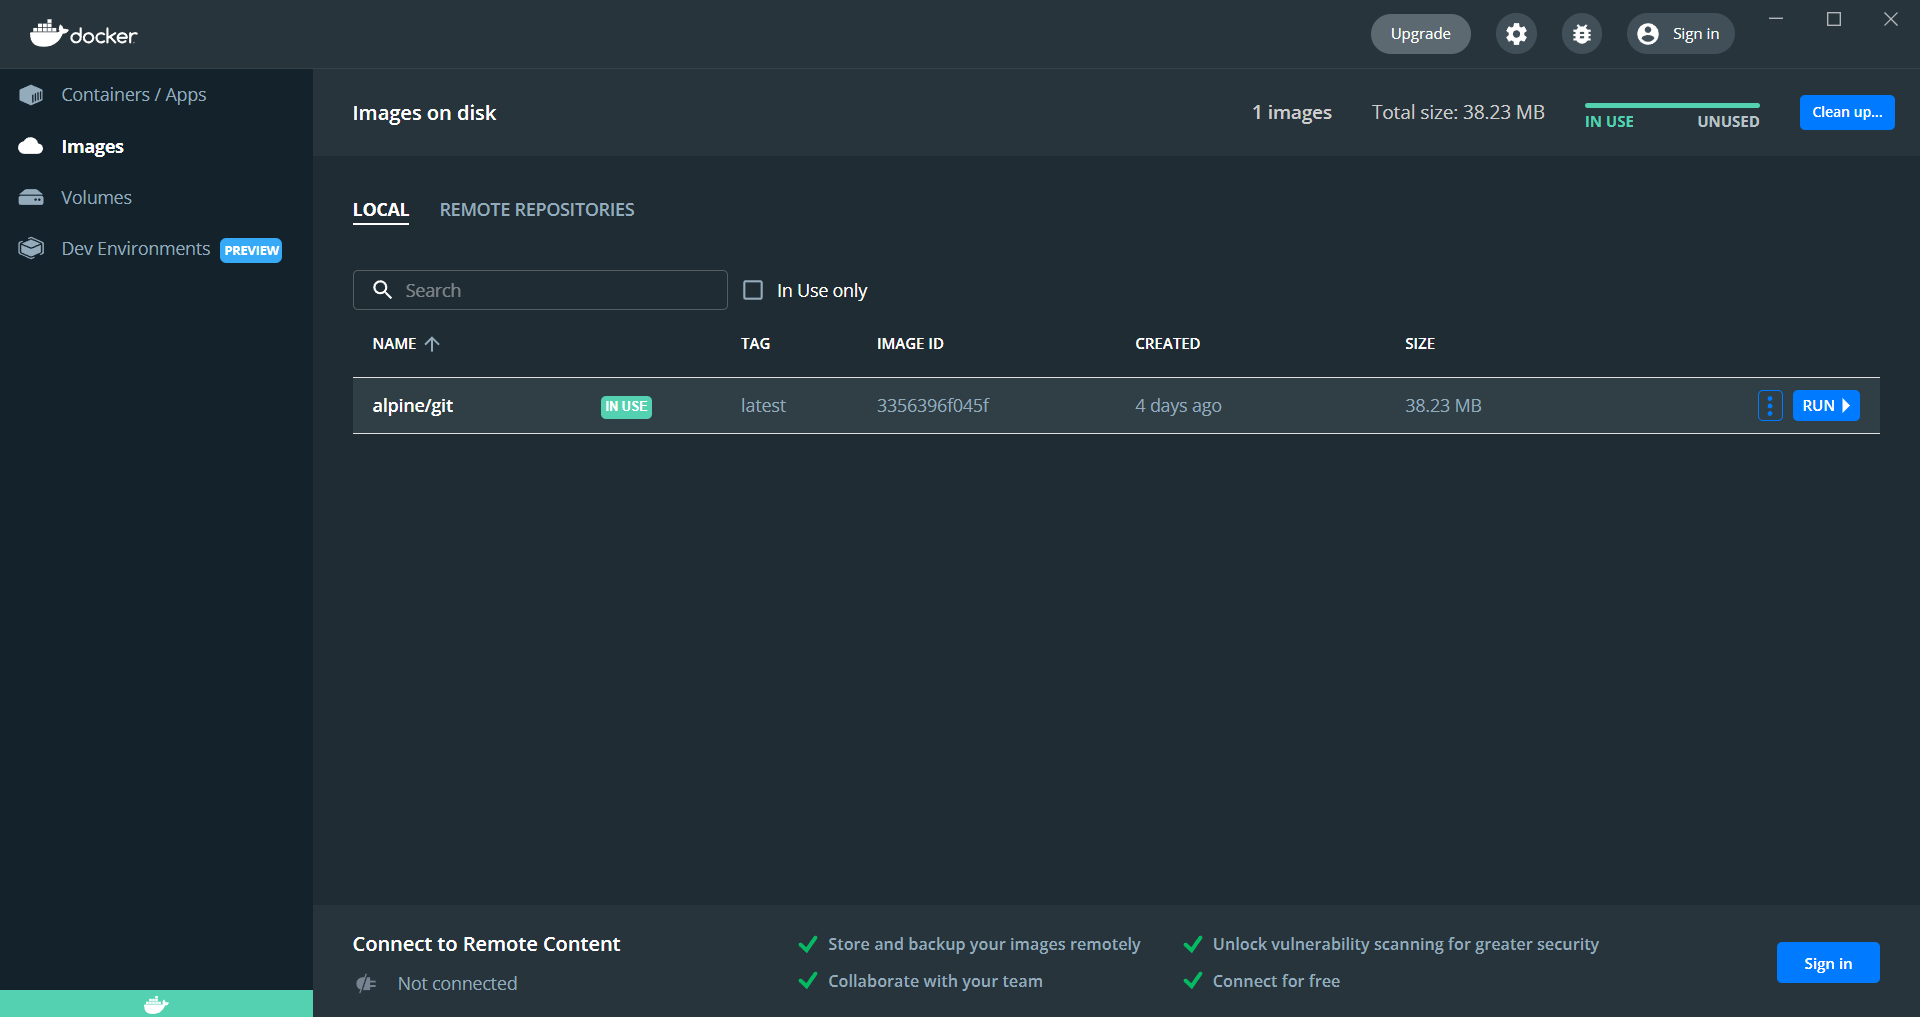
\includegraphics[width = 0.7\textwidth]{Figure/docker starting.png}
	\caption{Docker Sedang Starting}
\end{figure}
\newpage
\section{Percobaan}
\subsection{Hello-World}
Setelah Docker berhasil diInstall dan kita telah dapat menjalankan perintah Docker dengan menggunakan PowerShell atau Command Prompt kita dapat melakukan percobaan berikut.
kita akan mencoba hello world menggunakan Windows PowerShell dengan docker command sebagai berikut.
\begin{lstlisting}[language=bash]
	docker run hello-World
\end{lstlisting}
\begin{figure}[h]
	\centering
	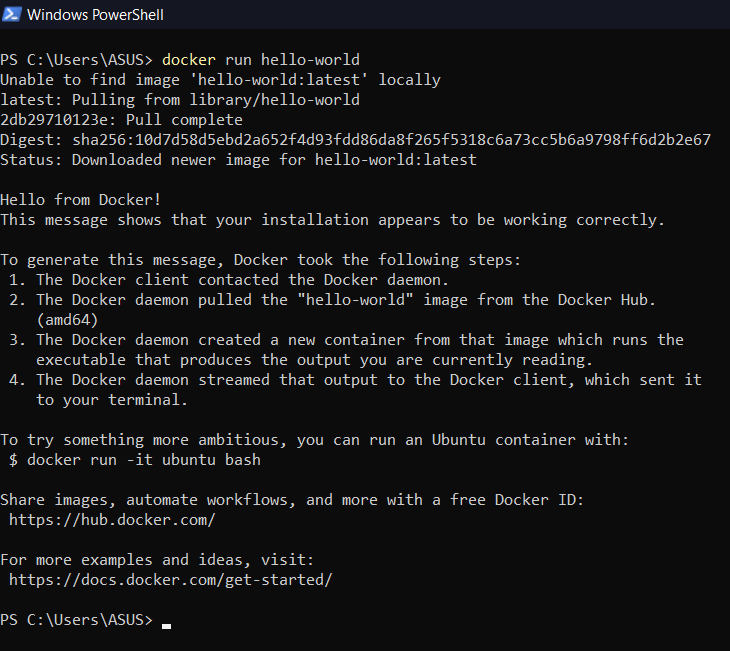
\includegraphics[width = 0.7\textwidth]{Figure/run hello-world.png}
	\caption{Docker run hello-world}
\end{figure}

\subsection{Alpine linux}
Langkah selanjunya kita akan coba membuka Windows PowerShell atau Command Prompt dan menjalankan container dari Alpin Linux dengan docker command berikut.
\begin{lstlisting}[language = bash]
	Docker Pull Alpine
\end{lstlisting}
\begin{figure}[h]
	\centering
	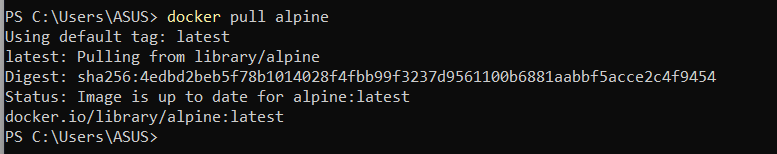
\includegraphics[width = 0.7\textwidth]{Figure/pullalpine.png}
	\caption{Docker Pull Alpine}
\end{figure}

\subsection{Docker Images}
Pada percobaan selanjutnya yaitu melakukan pengecekan semua image yang pernah kita pull atau unduh dengan menggunakan perintah berikut.
\begin{lstlisting}[language = bash]
	Docker images
\end{lstlisting}
\begin{figure}[h]
	\centering
	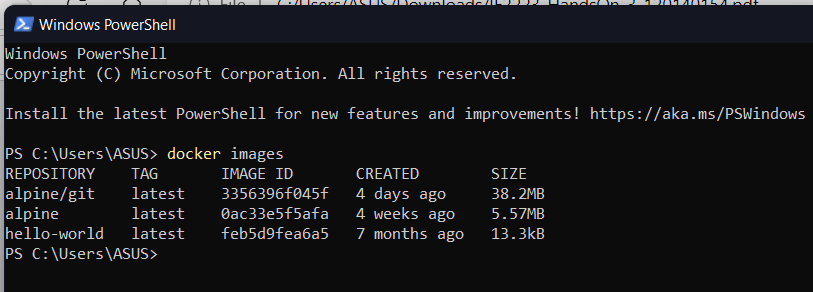
\includegraphics[width = 0.7\textwidth]{Figure/docker image.png}
	\caption{Docker run Image}
\end{figure}
Langkah berikutnya kita akan mencoba menjalankan salah satu Container dengan menggunakan perintah sebagai berikut
\begin{lstlisting}[language = bash]
	Docker run alpine ls -l
\end{lstlisting} 
\begin{figure}[h]
	\centering
	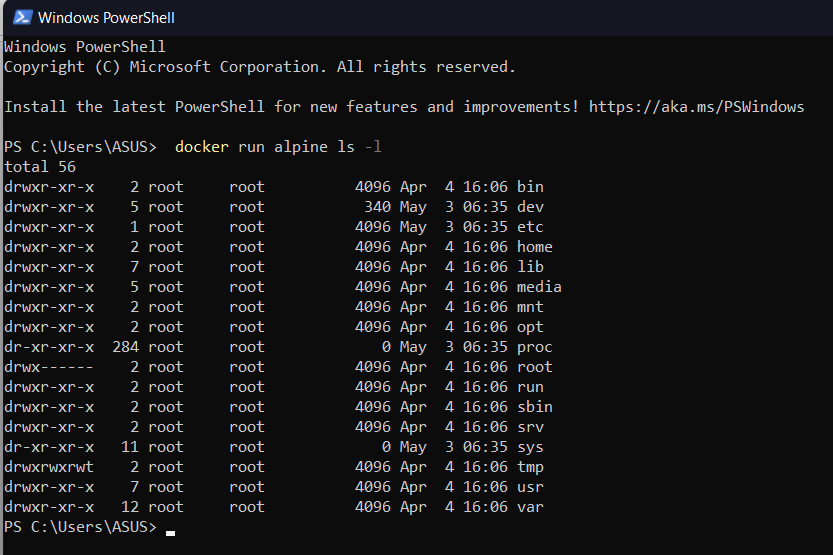
\includegraphics[width = 0.7\textwidth]{Figure/alpine -1.png}
	\caption{Docker Run Alpine ls -l}
\end{figure}
Setelah itu kita akan menampilkan kalimat pada windows powershell dengan command docker run alpine dan tambahan echo, echo disini sama fungsinya seperti linux. berikut commandnya
\begin{lstlisting}[language=bash]
	Docker run echo "Hello World"
\end{lstlisting}

\newpage
Selanjutnya kita akan mencoba masuk kedalam bash dari Container alpine tersebut dengan menggunakan perintah berikut.
\begin{lstlisting}[language = bash]
	Docker run alpine -it /bin/sh 
\end{lstlisting}
\begin{figure}[h]
	\centering
	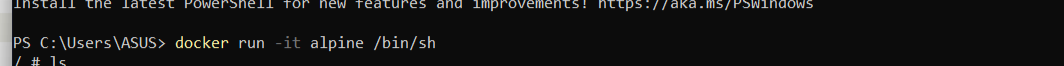
\includegraphics[width = 0.7\textwidth]{Figure/bash cont.png}
	\caption{Bash dari Container Alpine}
\end{figure}
Selanjutnya kita dapat menampilkan list dari seluruh file yang pada bin/sh dengan memberikan command atau perintah baru di dalam /bin/sh seperti berikut.
\begin{lstlisting}[language = bash]
	/ # ls
\end{lstlisting}
\begin{figure}[h]
	\centering
	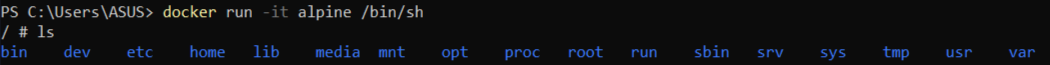
\includegraphics[width = 0.7\textwidth]{Figure/ls.png}
	\caption{List dari /bin/sh}
\end{figure}
Selanjutnya kita dapat menampilkan seluruh informasi dasar yang dimiliki oleh sistem dengan menggunakan command sebagai berikut.
\begin{lstlisting}[language = bash]
	/ # uname -a
\end{lstlisting}
\begin{figure}[h]
	\centering
	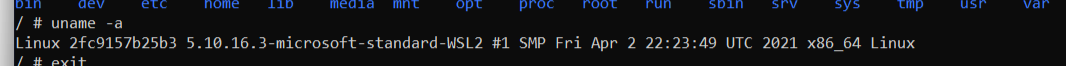
\includegraphics[width = 0.7\textwidth]{Figure/uname.png}
	\caption{Uname -a dari /bin/sh}
\end{figure}
Untuk keluar dari bash kita dapat menggunakan perintah berikut.
\begin{lstlisting}[language = bash]
	/ # exit
\end{lstlisting}
Kemudian untuk menampilkan \textit{container} yang telah dijalakan sebelumnya, dapat dilakukan dengan menggunakan perintah berikut.
\begin{lstlisting}[language = bash]
	Docker ps -a
\end{lstlisting}
\begin{figure}[h]
	\centering
	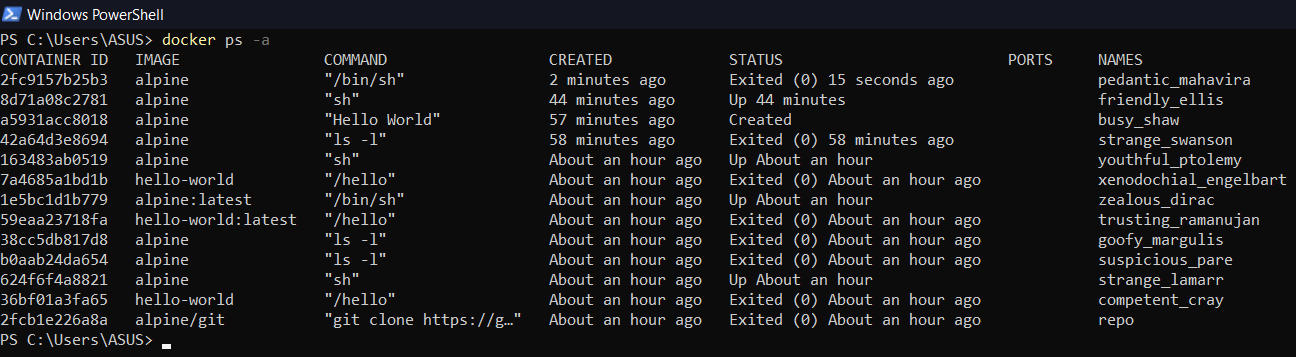
\includegraphics[width = 0.7\textwidth]{Figure/ps -a.png}
	\caption{Docker ps -a}
\end{figure}
\newpage
Kita dapat melihat container yang telah kita jalankan pada Aplikasi docker sebelumnya seperti gambar di bawah ini
\begin{figure}[h]
	\centering
	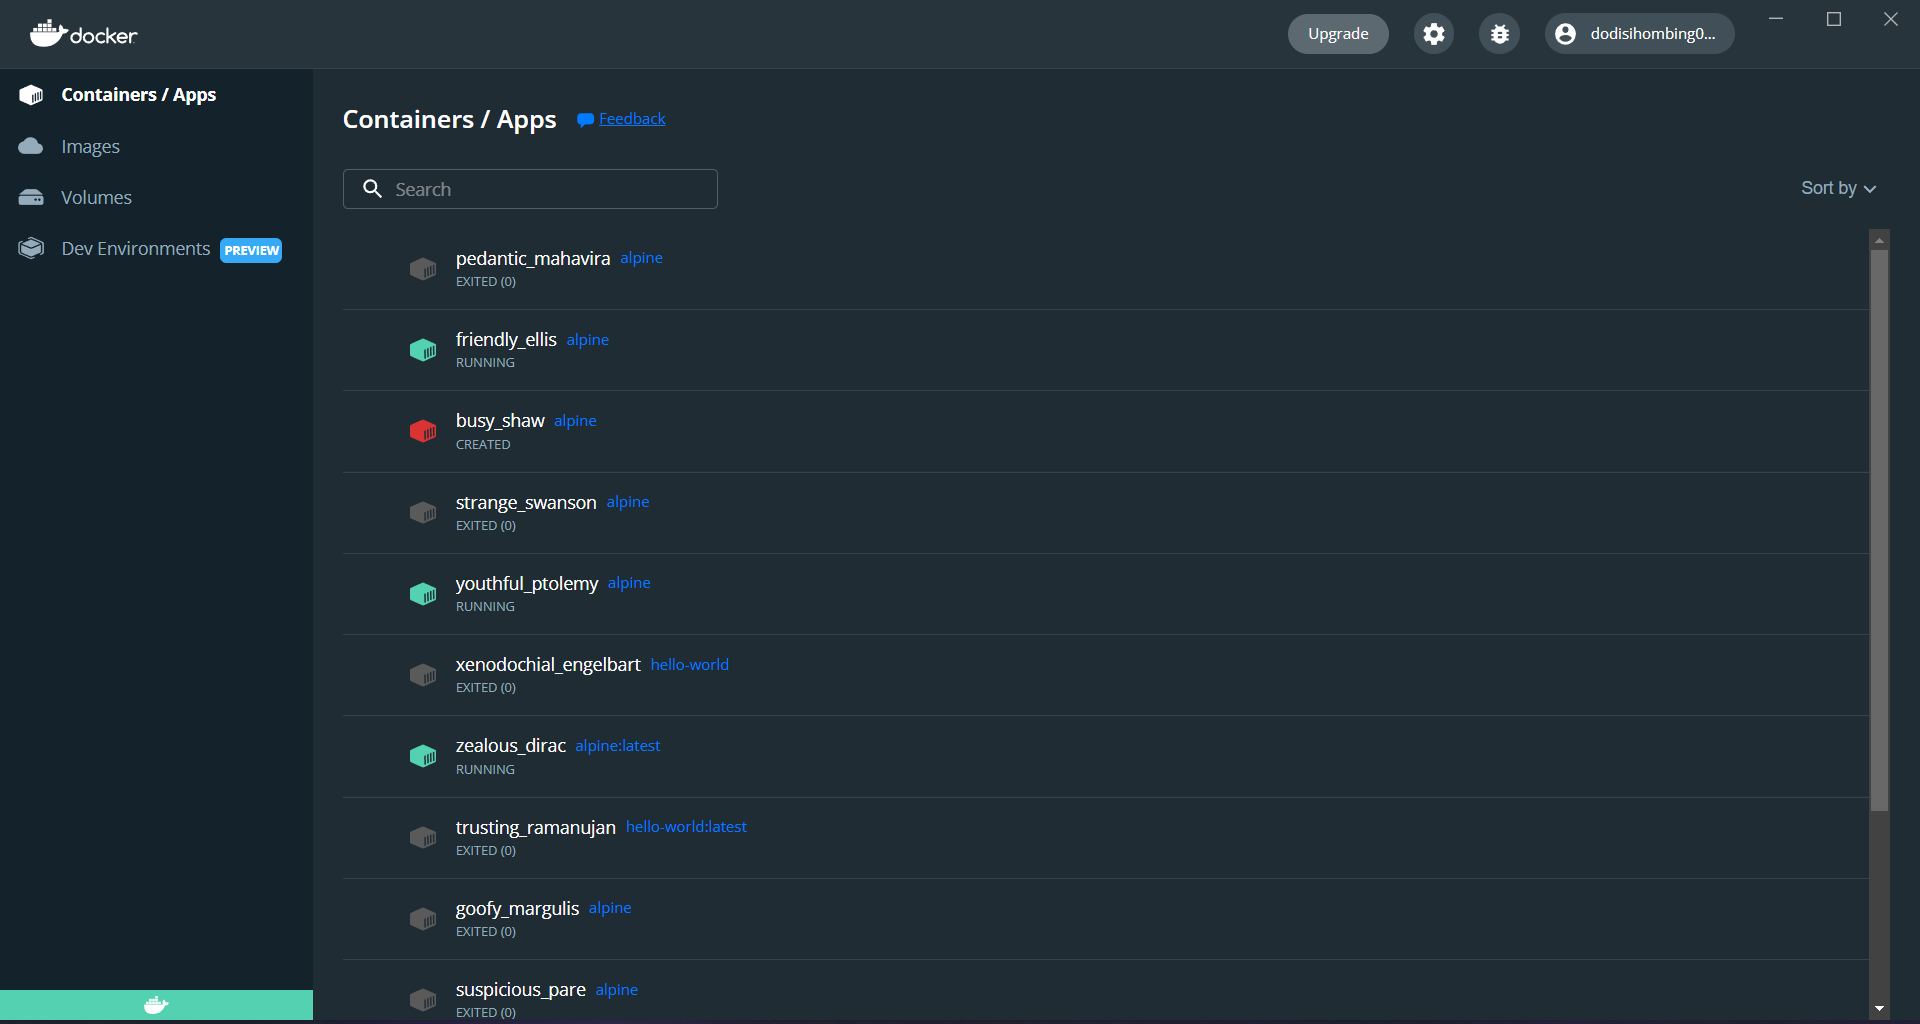
\includegraphics[width = 0.7\textwidth]{Figure/ps -a22.png}
	\caption{Riwayat Container Desktop}
\end{figure}
\section{Pertanyaan Hands On}
\subsection{Apa itu Docker}
Docker adalah sebuah layanan aplikasi yang berfugsi untuk menyediakan suatu kemampuan untuk mengemas dan menjalankan sebuah aplikasi dalam sebuah lingkungan yang terisolasi yang disebut dengan container. Dengan adanya isolasi dan keamanan yang memadai memungkinkan untuk menjalankan banyak container di waktu yang bersamaan pada host tertentu.\cite{shinta_2021}

\subsection{Apa fungsi dari perintah perintah "docker run"}
Perintah docker run digunakan untuk menjalankan proses dalam container yang terisolasi. Images yang
terdapat dalam container akan dieksekusi sesuai dengan konfigurasi yang akan dibuat. Ketika perintah docker
run dijalankan, image container akan dieksekusi seolah-olah Anda sedang menjalankan aplikasi. Biasanya,
memiliki beberapa port yang terbuka sehingga aplikasi di dalam container yang sedang berjalan dapat diakses
dari luar container
Container tersebut.\\
berikut Command yang dapat di gunakan untuk menjalankan sebuah Container:
\begin{lstlisting}[language = bash]
	docker run [image] #hanya menjalankan Containernya

	docker run [image] [Command] #menjalankan Container sekaligus Commandnya (contoh Command = echo)

	docker run [option] [image] [Command] #menjalankan image beserta option yang terdapat pada docker(Contoh option = -i)
\end{lstlisting}
kita juga dapat mencari option yang sesuai dengan kebutuhan kita dapat kita ketikan "docker run --help" yang di dalamnya terdapat banyak option yang disediakan.

\begin{figure}[h]
	\centering
	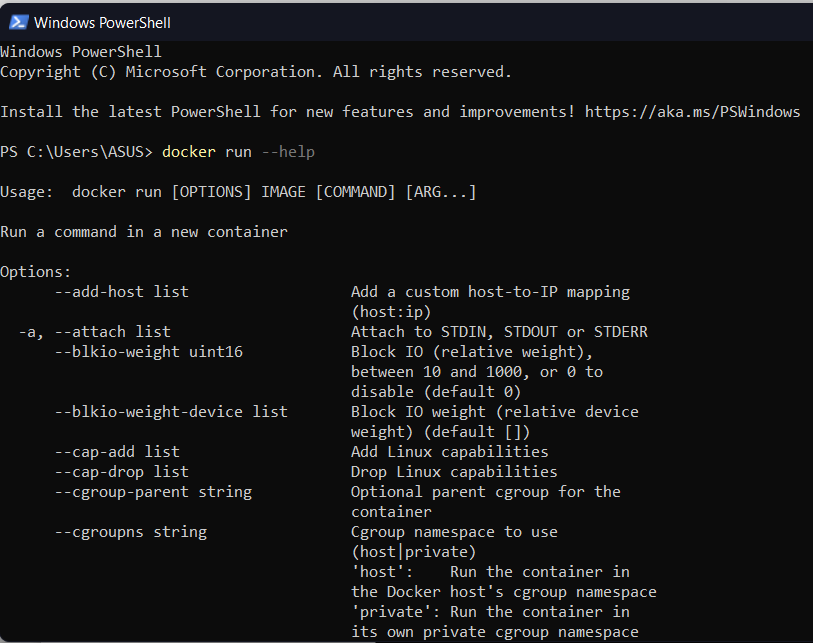
\includegraphics[width = 0.7\textwidth]{Figure/docker help.png}
	\caption{help untuk docker run}
\end{figure}

\subsection{Apa yang dimaksud dengan Conatainer}
Docker container adalah environment untuk mengemas aplikasi yang mencakup system tools, library,code, runtime dan konfigurasi. Container dapat juga dikatakan sebagai sebuah folder yang terisolasi. Container ini digunakan untuk 
membungkus images yang berupa aplikasi atau tools yang ingin di isolasi. 

\subsection{Apa fungsi dari perintah "docker ps -a"}

docker ps -a merupakan sebuah command docker yang berfungsi untuk menampilkan seluruh Container baik yang sedang berjalan maupun yang telah berhenti atau dapat menampilkan semua data container yang pernah
dibuat. Untuk "ps-a" menampilkan container id hingga names seperti gambar dibawah
\begin{lstlisting}[language = bash]
	docker ps -a
\end{lstlisting}
\begin{figure}[h]
	\centering
	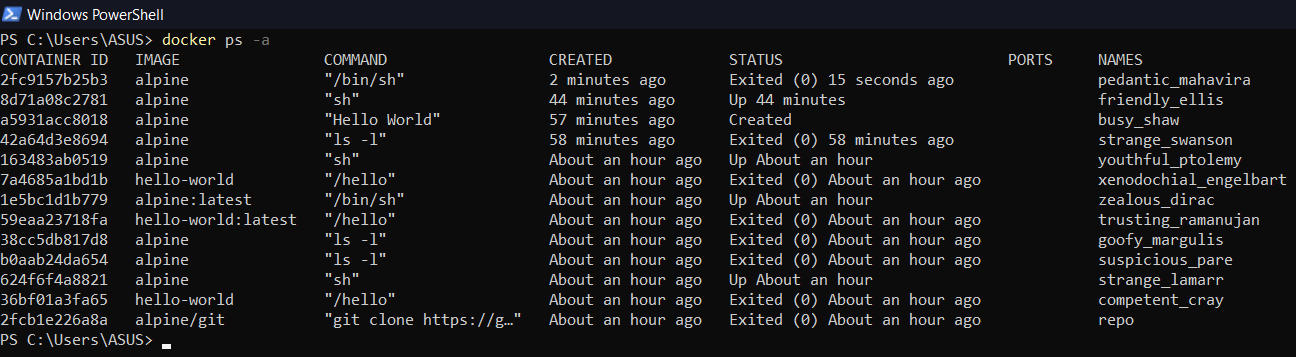
\includegraphics[width = 0.7\textwidth]{Figure/ps -a.png}
\end{figure}

\newpage
\subsection{Apa fungsi dari perintah "docker run -it"}
Docker run -it adalah sebuah command docker untuk mengalokasi sebuah pseudo-TTY atau bentuk komunikasi dua arah antara komputer utama dengan ruang yang terisolasi dengan membuat sebuah interactive
bash shell pada container. perintah yang digunakan sebagai berikut
\begin{figure}[h]
	\centering
	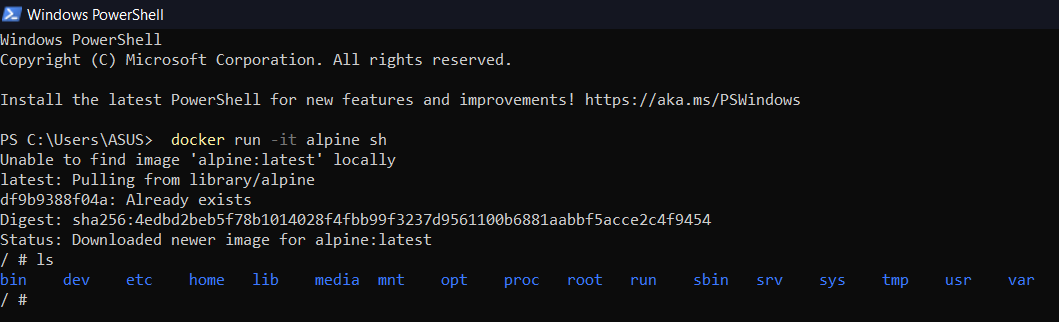
\includegraphics[width = 0.7\textwidth]{Figure/docker run it.png}
\end{figure}


\subsection{Apa yang dimaskud dengan images}
Docker images adalah file yang digunakan untuk mengeksekusi kode dalam Docker container.

\subsection{Apa yang dimaksud dengan deamon}
Docker daemon adalah sebuah service yang dijalankan di dalam host OS. Docker daemon ini berfunsi untuk
membangun, mendistribusikan, dan menjalankan container docker. kita tidak dapat secara lengsung mengakses docker daemon, akan tetapi untuk menggunakan docker daemon dapat menggunakan docker client sebagai perantara atau CLI.\cite{contributor_2005}
\section{Kesimpulan}
Dari Hands On 3 kali ini dapat disimpulkan bahwa Docker adalah sebuah sofware yang dapat memebantu developer dalam melakukan developing, shipping, dan running aplikasi melalui infrastruktur yang terpisah dari PC developer, sehingga resouce yang diperlukan dalam proses pengembangan aplikasi tersebut akan lebih sedikit.

\section{Link GitHub}
	Link GitHub dari Hands On 3 ini : \href{https://github.com/dodisihombing016/HandsOn-3}{Klik disini}

\newpage
\bibliographystyle{IEEEtran}
\bibliography{Referensi.bib}




\end{document}